% Assignment labels use hyphens; Russian list labels have unmatched closing parentheses.
% chktex-file 8
% chktex-file 17
% Ellipsis placement is handled by amsmath.
% chktex-file 11
\documentclass[a4paper,11pt]{article}
\usepackage{hometask}
\usepackage{amssymb}
\usepackage{tikz}
\usepackage{pdfpages}
\usetikzlibrary{arrows.meta,decorations.pathreplacing}

\setlength{\parindent}{0pt}
\setlength{\parskip}{5pt}
\setlength{\headheight}{24pt}

\newcommand{\hwheap}[1]{%
	\fill (0,0) circle (.65pt);
	\ifnum#1>0
		\pgfmathsetmacro{\spread}{.16 * 2 ^ (#1 - 1)}
		\pgfmathtruncatemacro{\nextdepth}{#1-1}
		\draw (0,0) -- (-\spread,-.3) (0,0) -- (\spread,-.3); % chktex 1
		\begin{scope}[shift={(-\spread,-.3)}]
			\hwheap{\nextdepth}
		\end{scope}
		\begin{scope}[shift={(\spread,-.3)}]
			\hwheap{\nextdepth}
		\end{scope}
	\fi
}

\begin{document}

{\large\bfseries 2-1.} Будем действовать так:

\begin{minipage}[t]{.53\textwidth}
	\vspace{0pt}
	1. Выбираем pivot (например, методом пятерок).

	2. За время $O(m+n)$ делаем partition отдельно для $n$ ключей и $m$ запросов
	(ключи разделяются по pivot-у, после чего известен размер левой части массива,
	по которому делятся запросы).
\end{minipage}\hfill
\begin{minipage}[t]{.44\textwidth}
	\vspace{0pt}
	\centering
	\begin{tikzpicture}[x=.82cm,y=.82cm,font=\scriptsize]
		\draw (0,0) -- (5.5,0);
		\foreach \x in {0,2.7,5.5} \draw (\x,-.12) -- (\x,.12);
		\node[below] at (1.2,-.15) {$K_{i_1},K_{i_2},\dots,K_{i_\ell}$};
		\node[below] at (2.7,-.15) {$p_1$};
		\node[below] at (4.3,-.15) {$K_{i_{\ell+1}},\dots,K_{i_m}$};
		\draw (0,-.65) to[out=-90,in=90] (-.25,-1.7);
		\draw (2.7,-.65) to[out=-90,in=90] (5.2,-1.7);
		\draw (0,-1.9) -- (4.9,-1.9);
		\foreach \x in {0,2.1,4.9} \draw (\x,-2.02) -- (\x,-1.78);
		\node[below] at (2.1,-2.02) {$p_2$};
		\node[below] at (1,-2.3) {$K_{j_1},\dots,K_{j_s}$};
		\node[below] at (3.9,-2.3) {$K_{j_{s+1}},\dots,K_{j_\ell}$};
		\draw (0,-2.8) to[out=-90,in=90] (-.25,-3.75);
		\draw[dashed] (2.1,-2.8) to[out=-90,in=90] (4.7,-3.75);
		\draw (0,-3.95) -- (4.4,-3.95);
		\foreach \x in {0,2,4.4} \draw (\x,-4.07) -- (\x,-3.83);
		\node[below] at (2,-4.07) {$p_3$};
	\end{tikzpicture}
\end{minipage}

3. Запускаем pivot + partition рекурсивно для всех частей, где есть запросы.
При условии, что запросы разные, на каждой итерации для всех частей, куда попадают запросы,
мы будем тратить не больше чем $O(n+m)$:

Если $C_i$ --- куски поделенного массива, $d_i$ --- число попадающих туда запросов.
$\sum C_i\leq n$, $\sum d_i=m$.
Время pivot + partition внутри каждого
\[
	O\Bigl(\sum(C_i+d_i)\Bigr)\approx O(n+m).
\]
\hrule
\medskip
Примерно за $\log_2 m$ итераций каждый из ключей получит <<свой>> кусок массива $C_i$.
В каждом из них статистика ищется линейно $\Rightarrow$
за время $O(\sum C_i)=O(n)$ ищутся все статистики.
\[
	\text{Итого}\qquad (m+n)\cdot\log_2 m+n
	\quad\Longrightarrow\quad O\bigl((m+n)\log m\bigr).
\]
Ну, немного хуже, чем требуется в задаче\dots

\newpage

{\large\bfseries 2-2.}

Будем поддерживать неупорядоченный массив размера $\leq 2k$.
Действовать будем так:
\begin{enumerate}
	\item Если размер массива $<2k$, то вставки <<бесплатные>>, просто добавляются в конец.
	\item При достижении размера $2k$ с помощью метода пятерок за время $O(2k)$ ищем медиану
	      и еще за время $O(2k)$ с помощью нее оставляем только $k$ элементов.
\end{enumerate}
\begin{center}
	\begin{tikzpicture}[x=.55cm,y=.65cm,>=Stealth,font=\small]
		\draw[->] (0,0) -- (18,0);
		\draw (0,-.2) -- (0,.3);
		\foreach \x in {1,...,14} {
				\draw (\x,0) -- (\x,-.12);
				\node at (\x,-.45) {$+$};
			}
		\node[below] at (7,-.65) {$k$};
		\node[below] at (14,-.65) {$2k$};
		\draw[->] (14,-1.15) -- (12.5,-1.8);
		\node[below] at (12,-1.8) {$\operatorname{compact},\ t=O(2k)$};
	\end{tikzpicture}
\end{center}

Для операций вставки суммарное время работы
\[
	t=\underbrace{n}_{\substack{\text{число вставок}\\\text{в конец}}}
	+\underbrace{\frac{n}{k}}_{\text{число <<сжатий>>}}
	\cdot\underbrace{4k}_{\substack{\text{стоимость}\\\text{сжатия}}}=5n.
\]
Тогда амортизированное время $\dfrac{t}{n}=5=O(1)$.

3. Get-Kth работает (с помощью того же метода пятерок) за время
$O(2k)\simeq O(k)$ в худшем случае, что и требуется в задаче.

\newpage

{\large\bfseries 2-3.}
\begin{center}
	\begin{tikzpicture}[>=Stealth,font=\small]
		\begin{scope}[scale=1.9]
			\hwheap{3}
		\end{scope}
		\node[above] at (0,.05) {$\min$};
		\draw[decorate,decoration={brace,mirror,amplitude=4pt}]
		(-2.2,-1.95) -- (2.2,-1.95) node[midway,below=6pt] {$n$ --- изначальная куча};
		\draw[->,thick] (1,.1) to[out=35,in=145] (3.2,.1);
		\begin{scope}[shift={(4.3,-.2)},scale=1.35]
			\draw (0,0) -- (-.45,-.5) -- (-.7,-.9)
			(-.45,-.5) -- (-.2,-.9) (0,0) -- (.45,-.5) -- (.2,-.9);
			\foreach \p in {(0,0),(-.45,-.5),(-.7,-.9),(-.2,-.9),(.45,-.5),(.2,-.9)}
			\draw[fill=white] \p circle (1pt);
		\end{scope}
		\draw[decorate,decoration={brace,mirror,amplitude=4pt}]
		(3.3,-1.65) -- (5.3,-1.65) node[midway,below=6pt] {$\leq k$};
		\node[right] at (5.5,-.7) {--- дополнительная куча};
	\end{tikzpicture}
\end{center}

Можно заметить, что при нахождении очередного минимума следующие кандидаты по минимуму ---
это все предыдущие кандидаты (кроме найденного) $+$ 2 его потомка:
\begin{center}
	\begin{tikzpicture}[>=Stealth,font=\scriptsize]
		\begin{scope}[scale=1.5]
			\hwheap{2}
		\end{scope}
		\node[above] at (0,.05) {$\min$};
		\draw[->,thick] (1.15,-.4) -- (2.35,-.4);
		\begin{scope}[shift={(3.6,0)},scale=1.5]
			\draw[dashed] (0,0) -- (-.32,-.3) (0,0) -- (.32,-.3);
			\draw (0,0) circle (.07);
			\begin{scope}[shift={(-.32,-.3)}] \hwheap{1} \draw (0,0) circle (.08); \end{scope}
			\begin{scope}[shift={(.32,-.3)}] \hwheap{1} \draw (0,0) circle (.08); \end{scope}
		\end{scope}
		\node[above] at (3.6,.25) {2 новых кандидата};
		\draw[->,thick] (4.6,-.4) -- (5.8,-.4);
		\begin{scope}[shift={(7.15,0)},scale=1.5]
			\draw[dashed] (0,0) -- (-.32,-.3) -- (-.56,-.6)
			(-.32,-.3) -- (-.08,-.6) (0,0) -- (.32,-.3);
			\draw (0,0) circle (.06) (-.32,-.3) circle (.06);
			\foreach \x/\y in {-.56/-.6,-.08/-.6,.32/-.3} {
					\begin{scope}[shift={(\x,\y)}]
						\hwheap{1}
						\draw (0,0) circle (.07);
					\end{scope}
				}
		\end{scope}
		\node[above] at (7.5,.25) {3 кандидата};
	\end{tikzpicture}
\end{center}

Используя этот факт, будем действовать так:
\begin{enumerate}
	\item Заведем вторую кучу. В ней будем хранить значения $+$ указатели на вершины изначальной кучи.
	\item В 0-й момент во второй куче корень из первой кучи.
	\item На каждой итерации (Get Next Min) делаем так:
	      \renewcommand{\labelenumii}{\arabic{enumii}.}
	      \begin{enumerate}
		      \item Извлекаем минимум из второй кучи за $t=\log(i)$, где $i$ --- ее размер.
		      \item Добавляем двух потомков извлеченного элемента за $2\cdot\log(i)$.
		            Размер кучи увеличился на 1.
	      \end{enumerate}
\end{enumerate}
Тогда время работы
\[
	\begin{aligned}
		T & =3\cdot\log(1)+3\cdot\log(2)+\dots+3\cdot\log(k) \\
		  & =3\log(k!)\approx 3k\log k=O(k\log k).
	\end{aligned}
\]

\newpage

{\large\bfseries 2-4.}

\begin{minipage}[t]{.34\textwidth}
	\vspace{0pt}
	\centering
	\begin{tikzpicture}[font=\small]
		\begin{scope}[scale=1.45]
			\draw (0,0) -- (-.64,-.3) -- (-.96,-.6) -- (-1.12,-.9)
			(-.96,-.6) -- (-.8,-.9) (-.64,-.3) -- (-.32,-.6) -- (-.48,-.9)
			(-.32,-.6) -- (-.16,-.9) (0,0) -- (.64,-.3) -- (.32,-.6) -- (.16,-.9)
			(.32,-.6) -- (.48,-.9) (.64,-.3) -- (.96,-.6);
			\foreach \x in {-1.12,-.8,-.48,-.16} {
					\draw[dashed] (\x,-.9) -- (\x-.08,-1.2) (\x,-.9) -- (\x+.08,-1.2);
				}
			\draw[dashed] (.96,-.6) -- (.8,-.9) (.96,-.6) -- (1.12,-.9);
			\draw[gray] (0,.15) .. controls (-.7,.05) and (-1.7,-.75) .. (-1.35,-1.02)
			.. controls (-.8,-1.2) and (.6,-.65) .. (1.25,-.65)
			.. controls (1.65,-.35) and (.65,.25) .. (0,.15);
			\draw[gray,rotate=8] (0,-1.18) ellipse (1.35 and .23);
		\end{scope}
		\node at (1.95,-.1) {$n$};
		\node at (1.95,-1.65) {$k$};
	\end{tikzpicture}
\end{minipage}\hfill
\begin{minipage}[t]{.63\textwidth}
	\vspace{0pt}
	1) Если $k>\dfrac{n}{2}$, то достаточно запустить обычный Heapify % chktex 10
	(Sift Down начиная с нижних вершин).
	Он работает за
	\[
		O(n+k)<O(3k)=O(k).
	\]
\end{minipage}

2) Если $k\leq\dfrac{n}{2}$, то будем запускать Sift Down только начиная с предков % chktex 10
\underline{новых} вершин. Остальная часть кучи уже корректная. Это даст время
\[
	t=\frac{k}{2}\cdot 1+\frac{k}{4}\cdot 2+\frac{k}{8}\cdot 3+\dots\approx 2k=O(k).
\]
Проблема, что такая оценка сойдется на \underline{не-корневой} вершине:

\begin{minipage}[c]{.31\textwidth}
	\centering
	\begin{tikzpicture}[font=\small,>=Stealth,scale=.98]
		\begin{scope}[scale=1.4]
			\hwheap{3}
			\draw[very thick] (-.96,-.6) circle (.09);
			\draw[dashed,->] (-1.2,-.65) -- (-.72,-.2) -- (-.12,.12);
			\draw[dashed] (-1.12,-.9) -- (-1.2,-1.2) (-1.12,-.9) -- (-1.04,-1.2)
			(-.8,-.9) -- (-.88,-1.2) (-.8,-.9) -- (-.72,-1.2);
		\end{scope}
		\draw[decorate,decoration={brace,amplitude=4pt}] (1.85,-1.3) -- (1.85,.05)
		node[midway,right=5pt] {$\log n$};
		\draw[decorate,decoration={brace,mirror,amplitude=4pt}] (-1.8,-1.85) -- (-.9,-1.85)
		node[midway,below=5pt] {$k$};
	\end{tikzpicture}
\end{minipage}\hfill
\begin{minipage}[c]{.66\textwidth}
	Вершина, на которой оценка $\dfrac{k}{2^i}$ сломается, так как она не
	корневая.
	Для нее нужно <<доделать>> работу высоты не более чем $\log n$,
	то есть запустить Sift Down $\log n$ раз:
\end{minipage}
\begin{center}
	\begin{minipage}{.27\textwidth}
		\centering
		\begin{tikzpicture}[font=\small]
			\begin{scope}[scale=1.2]
				\hwheap{3}
				\draw[dashed] (-1.12,-.9) -- (-1.2,-1.2) (-1.12,-.9) -- (-1.04,-1.2);
			\end{scope}
			\draw[decorate,decoration={brace,amplitude=3pt}] (-1.6,.05) -- (-1.6,-.65)
			node[midway,left=4pt] {$\log n$};
			\draw[decorate,decoration={brace,amplitude=3pt}] (-1.6,-.7) -- (-1.6,-1.5)
			node[midway,left=4pt] {$\log k$};
		\end{tikzpicture}
	\end{minipage}\hfill
	\begin{minipage}{.7\textwidth}
		\[
			\begin{aligned}
				t & =\log k+(1+\log k)+(2+\log k)+{}                \\
				  & \quad+\dots+\log(n+k)                           \\
				  & \leq\underbrace{\log 2n+\dots+\log 2n}_{\log n} \\
				  & \leq\log^2 2n=O(\log^2 n).
			\end{aligned}
		\]
	\end{minipage}
\end{center}
Итого: $O(k+\log^2 n)$.

\medskip
\hrule
\medskip
3) Чтобы улучшить оценку, вместо того чтобы запускать Sift Down ценой $\log n$, $\log n$ раз, % chktex 10
можно было бы сразу отсортировать весь путь этой вершины.
Путь наверх состоит из $\log n$ вершин. Путь вниз еще $\log k$.
Но какие именно вершины взять, неизвестно. (Sift Down может идти в любую сторону\dots)

Короче, я не решил это, но явно можно хитро отсортировать этот путь и получить
$\log(n)\cdot\log(\log(n))\dots$~:) % chktex 10

\newpage

{\large\bfseries 2-5.}

Структура: не более $\log n$ куч размеров $1,3,7,\dots,2^k-1$.
К примеру, для:
\begin{center}
	\begin{tikzpicture}[font=\small]
		\foreach \n/\y in {1/0,2/-1.05,3/-2.1,4/-3.15,5/-4.2,6/-5.25,7/-6.3} {
				\node[anchor=east] at (-.55,\y-.2) {$n=\n\ \Rightarrow$};
			}
		\hwheap{0}
		\begin{scope}[shift={(0,-1.05)}] \hwheap{0} \end{scope}
		\begin{scope}[shift={(.6,-1.05)}] \hwheap{0} \end{scope}
		\node[right] at (1,-1.05) {(две кучи)};
		\begin{scope}[shift={(0,-2.1)}] \hwheap{1} \end{scope}
		\begin{scope}[shift={(0,-3.15)}] \hwheap{1} \end{scope}
		\begin{scope}[shift={(.7,-3.15)}] \hwheap{0} \end{scope}
		\begin{scope}[shift={(0,-4.2)}] \hwheap{1} \end{scope}
		\begin{scope}[shift={(.7,-4.2)}] \hwheap{0} \end{scope}
		\begin{scope}[shift={(1.2,-4.2)}] \hwheap{0} \end{scope}
		\begin{scope}[shift={(0,-5.25)}] \hwheap{1} \end{scope}
		\begin{scope}[shift={(.9,-5.25)}] \hwheap{1} \end{scope}
		\begin{scope}[shift={(.2,-6.3)}] \hwheap{2} \end{scope}
		\foreach \n/\y in {8/0,9/-1.05,10/-2.1,11/-3.15,12/-4.2,13/-5.25,14/-6.3,15/-7.35} {
				\node[anchor=east] at (5,\y-.2) {$n=\n\ \Rightarrow$};
			}
		\foreach \y in {0,-1.05,-2.1,-3.15,-4.2,-5.25,-6.3} {
				\begin{scope}[shift={(5.8,\y)}] \hwheap{2} \end{scope}
			}
		\begin{scope}[shift={(6.65,0)}] \hwheap{0} \end{scope}
		\begin{scope}[shift={(6.65,-1.05)}] \hwheap{0} \end{scope}
		\begin{scope}[shift={(7.15,-1.05)}] \hwheap{0} \end{scope}
		\begin{scope}[shift={(6.85,-2.1)}] \hwheap{1} \end{scope}
		\begin{scope}[shift={(6.85,-3.15)}] \hwheap{1} \end{scope}
		\begin{scope}[shift={(7.5,-3.15)}] \hwheap{0} \end{scope}
		\begin{scope}[shift={(6.85,-4.2)}] \hwheap{1} \end{scope}
		\begin{scope}[shift={(7.5,-4.2)}] \hwheap{0} \end{scope}
		\begin{scope}[shift={(8,-4.2)}] \hwheap{0} \end{scope}
		\begin{scope}[shift={(6.85,-5.25)}] \hwheap{1} \end{scope}
		\begin{scope}[shift={(7.65,-5.25)}] \hwheap{1} \end{scope}
		\begin{scope}[shift={(7.15,-6.3)}] \hwheap{2} \end{scope}
		\begin{scope}[shift={(6.5,-7.35)}] \hwheap{3} \end{scope}
	\end{tikzpicture}
\end{center}
То есть раскладываем $n$ по слагаемым $2^k-1$.
В каждый момент времени число куч одного размера не больше 2,
а все остальные кучи убывают как степень 2.
$\Rightarrow$ число куч $\approx\log n$.

\medskip
\hrule
\medskip
Extract Min:
\begin{enumerate}
	\item За $\log(n)$ находим минимальный элемент среди $\log n$ корней куч.
	\item За $O(1)$ разрываем кучу и отдаем корень.
	\item Если структура куч нарушилась, ее надо восстановить
	      (к примеру, <<разобрать>> наименьшую кучу за $O(1)$)
	      и использовать освободившийся элемент, чтобы восстановить предыдущую за $\log n$.
\end{enumerate}
Пример: $n=29$.
\begin{center}
	\begin{tikzpicture}[>=Stealth,font=\scriptsize,scale=.9]
		\begin{scope}[shift={(0,0)}]
			\hwheap{3}
			\draw (0,0) circle (.13);
		\end{scope}
		\node[above] at (0,.2) {$\min$};
		\begin{scope}[shift={(1.8,-.3)}] \hwheap{2} \end{scope}
		\begin{scope}[shift={(3,-.3)}] \hwheap{2} \end{scope}
		\draw[->,thick] (3.7,-.5) -- (4.4,-.5);
		\begin{scope}[shift={(5.2,-.3)}] \hwheap{2} \end{scope}
		\begin{scope}[shift={(6.4,-.3)}] \hwheap{2} \end{scope}
		\begin{scope}[shift={(7.6,-.3)}] \hwheap{2} \end{scope}
		\begin{scope}[shift={(8.8,-.3)}] \hwheap{2} \draw (0,0) circle (.13); \end{scope}
		\draw[dashed] (5.8,.05) circle (.12);
		\draw[dashed,->] (8.6,-.05) -- (6,.05);
		\node[above] at (6.8,.15) {отдаем};
		\draw[->,thick] (9.5,-.5) -- (10.2,-.5);
		\begin{scope}[shift={(11.3,0)}] \hwheap{3} \draw (0,0) circle (.13); \end{scope}
		\node[above] at (11.5,.2) {Sift Down};
		\begin{scope}[shift={(13.1,-.3)}] \hwheap{2} \end{scope}
		\begin{scope}[shift={(14.3,-.6)}] \hwheap{1} \end{scope}
		\begin{scope}[shift={(15,-.6)}] \hwheap{1} \end{scope}
	\end{tikzpicture}
\end{center}
\[
	\text{Итого:}\quad
	\underbrace{\log n}_{\text{найти мин.}}+
	\underbrace{1+1}_{\text{разобрать}}+
	\underbrace{\log n}_{\text{Sift Down}}=O(\log n).
\]

\newpage

Добавить элемент: элемент всегда добавляется

а) либо в новую кучу; % chktex 10

б) либо, если есть 2 одинаковые кучи, на них корень и запускается Sift Down. % chktex 10

Посчитаем амортизированную сложность.

Пусть $n=2^k-1$.
Тогда мы 1 раз делали слияние стоимостью $k$, 2 раза стоимостью $k-1$,
4 раза стоимостью $k-2$, \dots, $2^{k-1}$ раз стоимостью 0.
\[
	\begin{aligned}
		\text{Итого:}\quad t
		 & =2^0\cdot k+2^1(k-1)+4(k-2)+\dots+2^{k-1}\cdot 1 \\
		 & \approx\sum 2^i\cdot k-\sum 2^i\cdot i           \\
		 & =(k\cdot 2^k-k)-(k\cdot 2^k-2^{k+1}+2)           \\
		 & \approx 2^{k+1}\approx n=O(n).
	\end{aligned}
\]
Амортизированно $\dfrac{n}{n}\to O(1)$.

\newpage

{\large\bfseries 2-6.}
\[
	\left.
	\begin{gathered}
		h\in\mathcal{H},\qquad h\colon X\to\{0,\dots,m\}, \\
		P\bigl(h(x_1)=y_1,\dots,h(x_k)=y_k\bigr)\leq\frac{C}{m^k}
	\end{gathered}
	\right\}\quad (C,k)\text{-независимость}.
\]
\hrule
\[
	h(x)=\bigl((a_0+a_1x+\dots+a_{k-1}x^{k-1})\bmod p\bigr)\bmod m,
	\qquad p>m,
\]
$p$ --- простое.
\[
	\forall k\ \exists C\colon\ \forall m,p\quad\{h(x)\}\text{ --- $(C,k)$-независимые}.
\]
\hrule
\medskip
$P\bigl(h(x_1)=y_1,\dots,h(x_k)=y_k\bigr)\leq\dfrac{C}{m^k}$ можно переписать как
\[
	\max_{\vec{x},\vec{y}}\frac{\#\,h(\vec{x})=\vec{y}}{|\mathcal{H}|}
	\leq\frac{C}{m^k},
	\qquad\text{где } h(\vec{x})=\begin{pmatrix}h(x_1)\\\vdots\\h(x_k)\end{pmatrix}.
\]
$|\mathcal{H}|\approx p^k$ (каждый коэффициент $a_i$ принимает $p$ возможных значений).
\[
	\Rightarrow\quad\max_{\vec{x},\vec{y}}\#\,h(\vec{x})=\vec{y}
	\leq C{\left(\frac{p}{m}\right)}^k.
\]
\[
	h(\vec{x})=\vec{y}\quad\Longleftrightarrow\quad
	\begin{cases}
		(a_0+a_1x_1+\dots+a_{k-1}x_1^{k-1})\bmod p=y_1+i_1m, \\
		\hfill\vdots\hfill                                   \\
		(a_0+a_1x_k+\dots+a_{k-1}x_k^{k-1})\bmod p=y_k+i_k m.
	\end{cases}
\]
Система линейных уравнений с $k$ неизвестными $(a_0,\dots,a_{k-1})$ в поле $F_p$.
Ее определитель --- определитель Вандермонда
\[
	|A|=\prod_{1\leq i<j\leq k}(x_j-x_i)\ne 0
\]
по условию, так как $x_i$ различны.
$\Rightarrow$ для конкретных $\{i_1,\dots,i_k\}$ $\exists!$ решение. % chktex 40
Сами $i_\ell\in\bigl\{0;\lfloor\frac{p}{m}\rfloor\bigr\}$,
то есть всего наборов $|\{i_\ell\}|\simeq{\bigl(\lfloor\frac{p}{m}\rfloor+1\bigr)}^k$.
Таким образом,
\[
	\#\,h(\vec{x})=\vec{y}\leq{\left(\left\lfloor\frac{p}{m}\right\rfloor+1\right)}^k
	\leq 2^k{\left(\frac{p}{m}\right)}^k.
\]
Взяв $C=2^k$, получим, что $\#\,h(\vec{x})=\vec{y}\leq C{\left(\dfrac{p}{m}\right)}^k$.

\newpage

{\large\bfseries 2-7.}

$h\in\mathcal{H}$ --- $C$-универсально, если
$\forall x,y\quad P\bigl(h(x)=h(y)\bigr)\leq\dfrac{C}{m}$.
\[
	h\colon X\to\{0,\dots,m-1\}.
\]
\hrule
\[
	X\in\{0,\dots,2^w-1\},\qquad
	h_a(x)=\left\lfloor\frac{(ax)\bmod 2^w}{2^{w-\ell}}\right\rfloor.
\]
\begin{center}
	\begin{tikzpicture}[font=\small]
		\node at (0,0) {$a=$};
		\node (a) at (2,0) {$\underline{1}\ \underline{0}\ \underline{1}\ \underline{1}\
				\underline{0}\ \underline{1}\ \underline{0}\ \underline{1}$};
		\node at (4,0) {$\cdot$};
		\node (x) at (6,0) {$\underline{1}\ \underline{0}\ \underline{0}\ \underline{1}\
				\underline{1}\ \underline{0}\ \underline{1}$};
		\node[above] at (6,.2) {$x$};
		\node at (7.7,0) {$=$};
		\node at (9.8,0) {$\_\ \_\ \_\ \_\ \_\ \_\ \_$};
		\draw[decorate,decoration={brace,mirror,amplitude=4pt}] (.5,-.35) -- (3.5,-.35)
		node[midway,below=5pt] {$w$};
		\draw[decorate,decoration={brace,mirror,amplitude=4pt}] (4.6,-.35) -- (7.4,-.35)
		node[midway,below=5pt] {$w$};
		\draw[decorate,decoration={brace,amplitude=3pt}] (8.5,.4) -- (10,.4)
		node[midway,above=4pt] {$\ell$};
		\draw[decorate,decoration={brace,amplitude=3pt}] (10,.4) -- (11.2,.4)
		node[midway,above=4pt] {$w-\ell$};
		\draw[decorate,decoration={brace,mirror,amplitude=4pt}] (8.5,-.35) -- (11.2,-.35)
		node[midway,below=5pt] {$w$};
		\node[below] at (9.3,-1) {результат --- старшие $\ell$ битов};
	\end{tikzpicture}
\end{center}
$a\in\{0,\dots,2^w-1\}$, $a$ --- нечетно.

\medskip
\hrule
\medskip
Исходное условие переписывается как
\[
	\frac{\#\bigl(h(x)=h(y)\bigr)}{|\mathcal{H}|}\leq\frac{C}{2^\ell}
	\quad\Longleftrightarrow\quad
	\#\bigl(h(x)=h(y)\bigr)\leq C\frac{2^w/2}{2^\ell}=C\cdot 2^{w-\ell-1}.
\]
\hrule
\[
	h(x)=h(y)\quad\Longleftrightarrow\quad
	(ax-ay)\mathbin{\texttt{>{}>}}(w-\ell)=0
	\quad\Longleftrightarrow\quad a(x-y)=b,
\]
где старшие $\ell$ битов $b$ --- нули.

Известно, что $az=b$ имеет единственное решение для $a$, если $z$ --- нечетно.
Пусть $(x-y)=z\cdot 2^q$, $z$ --- нечетно.
\[
	\Rightarrow\quad az\cdot 2^q=b\pmod{2^w}
	\quad\Rightarrow\quad b=2^q\cdot b_1
\]
($b_1$ может быть и четным);
\[
	b=\underbrace{0\,0\,0\,0\,0}_{\ell}\dots\underbrace{0\,0\,0}_{q}.
\]
Тогда $az=b_1$ имеет единственное решение для $a$ в арифметике $w-q$.
Всего решений в изначальной арифметике $2^q$
(так как старшие $q$ бит для $a$ перестают влиять на результат из-за сдвига $2^q$).

$\Rightarrow\ \forall x,y$ число решений уравнения $a(x-y)=b$ в $2^w$ арифметике равно
\[
	\underbrace{2^q}_{\text{четность }(x-y)}\cdot
	\underbrace{2^{w-\ell-q}}_{\text{число подходящих }b}\cdot
	\underbrace{\frac{1}{2}}_{\substack{\text{из них нечетных }b_1\\\text{(так как $a$ --- нечетно)}}}
		=2^{w-\ell-1}.
\]
\[
	\Rightarrow\quad\#\bigl(h(x)=h(y)\bigr)=2^{w-\ell-1}
	\quad\Rightarrow\quad C\simeq 1.
\]

\clearpage
\makeatletter
\lastpage@putlabel % chktex 1
\let\lastpage@putlabel\relax
\makeatother
{
	\hoffset=0pt
	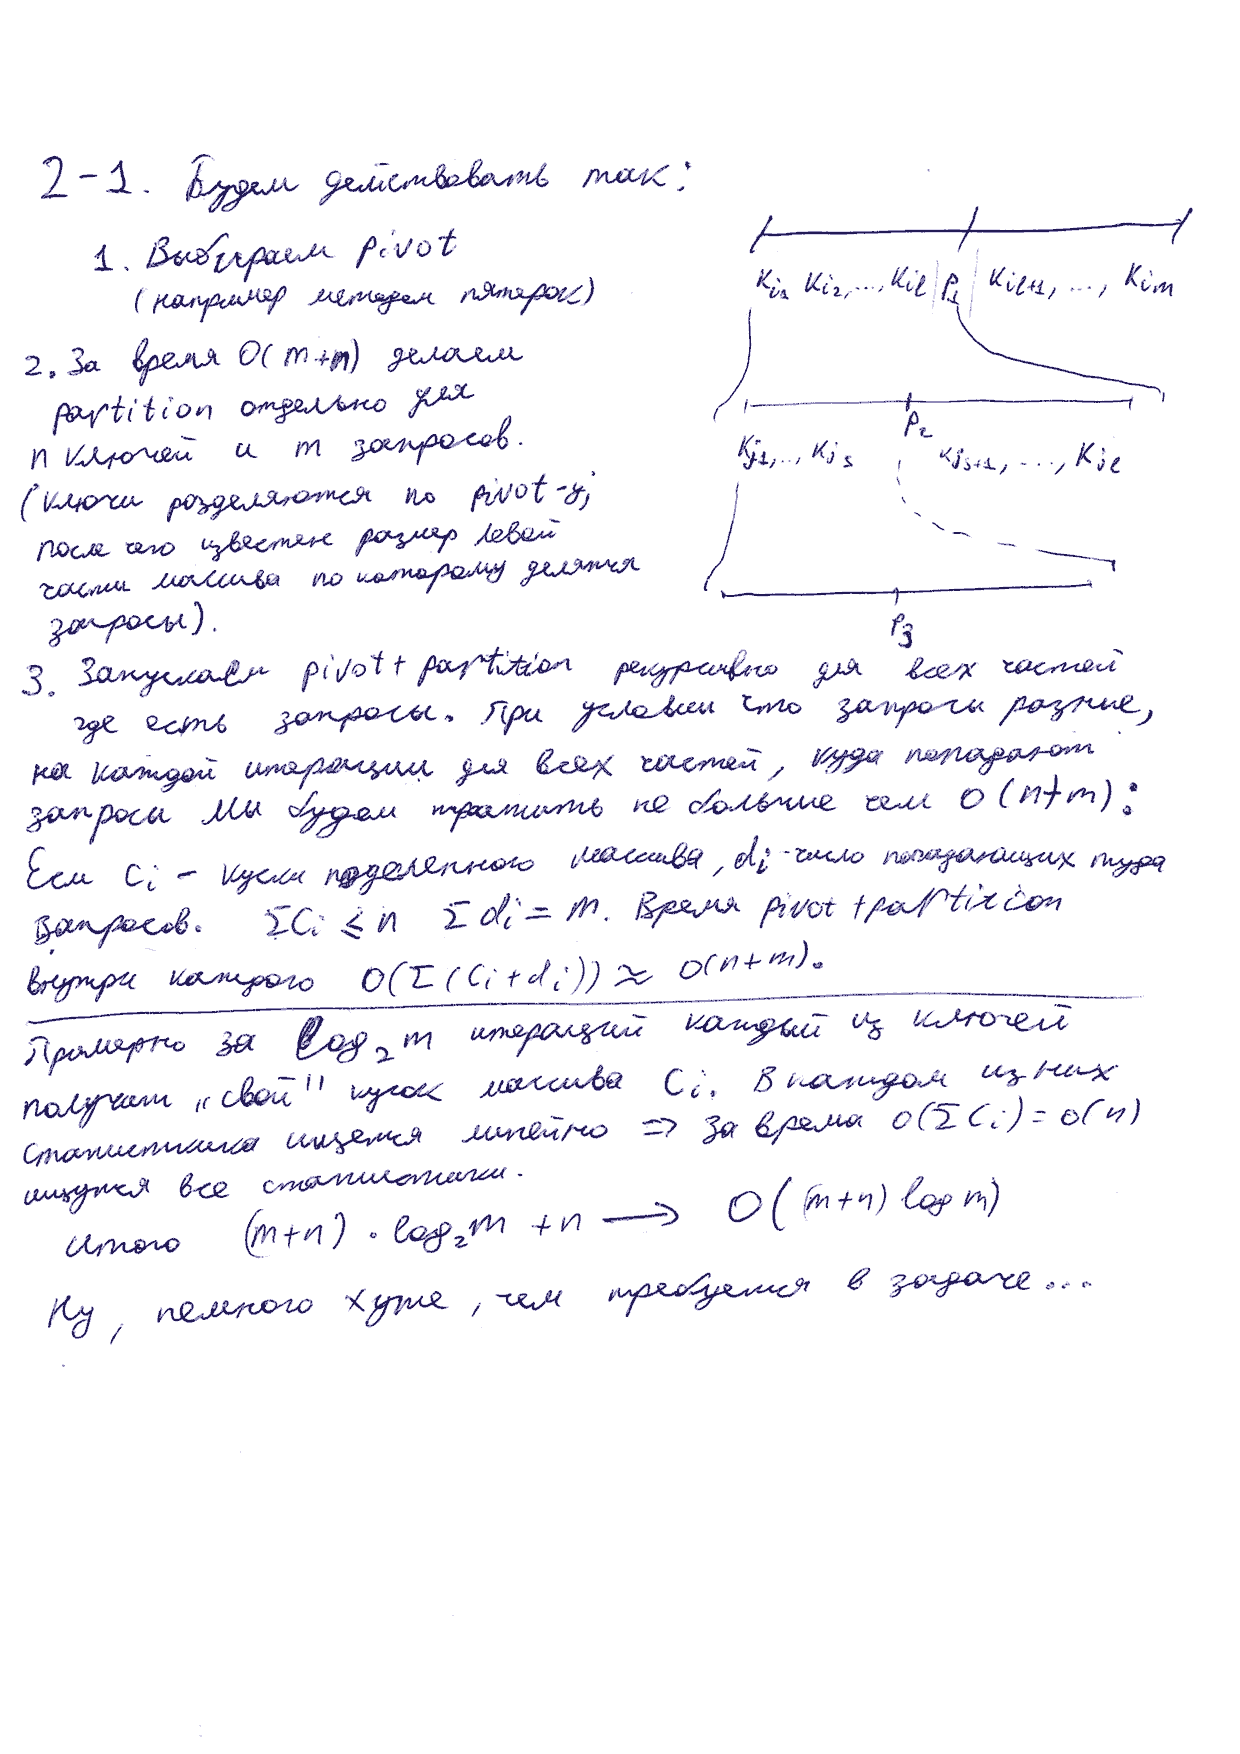
\includepdf[pages=-]{handwritten-2.pdf}
}

\end{document}
